\documentclass{article}
\usepackage[utf8]{inputenc}
\usepackage[portuguese]{babel}
\usepackage[margin=2.5cm]{geometry}
\setlength{\parskip}{1mm}
\setlength{\parindent}{10mm}
\linespread{1.2}
\usepackage[usenames,dvipsnames,svgnames,table]{xcolor}
\usepackage{fancyhdr}
\usepackage[symbol]{footmisc}
\usepackage{amsfonts,amsmath,amssymb,amsthm}
\newtheorem{thm}{Teorema}[]
\usepackage{array,caption,graphicx}
\usepackage[shortlabels]{enumitem}
\usepackage{verbatim}
\usepackage{listings}
\usepackage{float}
\usepackage{graphicx}
\definecolor{codegreen}{rgb}{0,0.6,0}
\definecolor{codegray}{rgb}{0.5,0.5,0.5}
\definecolor{codepurple}{rgb}{0.58,0,0.82}
\definecolor{backcolour}{rgb}{0.95,0.95,0.92}
\lstdefinestyle{mystyle}{
  backgroundcolor=\color{backcolour},   commentstyle=\color{codegreen},
  keywordstyle=\color{magenta},
  numberstyle=\tiny\color{codegray},
  stringstyle=\color{codepurple},
  basicstyle=\footnotesize,
  breakatwhitespace=false,
  breaklines=true,
  captionpos=b,
  keepspaces=true,
  numbers=left,
  numbersep=5pt,
  showspaces=false,
  showstringspaces=false,
  showtabs=false,
  tabsize=2
}
\renewcommand{\thefootnote}{\arabic{footnote}}
\lstset{style=mystyle}


\title{\textbf{Análise Numérica\\Relatório 4 - Cálculo de Integrais}}
\author{\textbf{Grupo 29}\\[4mm]José Dias\\Luís Pinto\\Samuel Neves\\Bárbara Gonçalves\\}
\date{22 de Maio de 2019}
\begin{document}
\maketitle
\clearpage
\pagestyle{fancy}
\fancyhf{}
\setlength{\headheight}{30pt}
\rhead{Relatório nº4}
\lhead{\textbf{Grupo 29}}
\setlength{\footskip}{15pt}
\rfoot{\thepage}
\section{Introdução}
\hspace{6mm}Com este trabalho pretendemos determinar o valor aproximado de $ I = \int_{0}^{1}\frac{\cos(x)^{30}}{\sin(x)^{30}+\cos(x)^{30}} $ tendo em conta a majoração do erro. Dito isto, alguns pontos a ter em consideração quanto ao mesmo:
\begin{enumerate}
  \item{O valor exato de  $ I = \int_{0}^{1}\frac{\cos(x)^{30}}{\sin(x)^{30}+\cos(x)^{30}} = 0.785398138155361 $, com um erro de $7\times10^{-14}$, foi obtido recorrendo ao  software Maxima}
  \item{A linguagem utilizada foi Python e, portanto, os cálculos foram feitos em dupla precisão.}
  \item{Para a resposta ao problema em questão serão usados alguns dos seguintes métodos:}
  \begin{enumerate}
    \item[\textbullet]{Resolução Teórica;}
    \item[\textbullet]{Código do programa;}
    \item[\textbullet]{Gráficos;}
    \item[\textbullet]{Tabelas;}
    \item[\textbullet]{Comentários.}

  \end{enumerate}
\end{enumerate}
\section*{Exercício 1.}
\textbf{Código utilizado:}
\begin{lstlisting}[language=Python]
from math import *
import time

def I_r(eps):
    start = time.time()
    a = float(input('Extremo esquerdo (a): '))
    b = float(input('Extremo direito (b): '))
    maxi = float(input('Maximo da derivada em [a,b]: '))
    n = int(((b-a)**2)/(2*eps)*maxi)+1
    soma = 0
    print('n =',n)
    for i in range(n):
        soma += (f(a+i*abs((a-b))/n)*(abs(a-b)/n))
    print('Integral =',soma,'Tempo de execucao:',time.time()-start)
def f(x):
    return cos(x)**30/(sin(x)**30+cos(x)**30)
\end{lstlisting}
\newpage
\flushleft{\textbf{Gráfico:}}
\begin{figure}[H]
  \begin{center}
    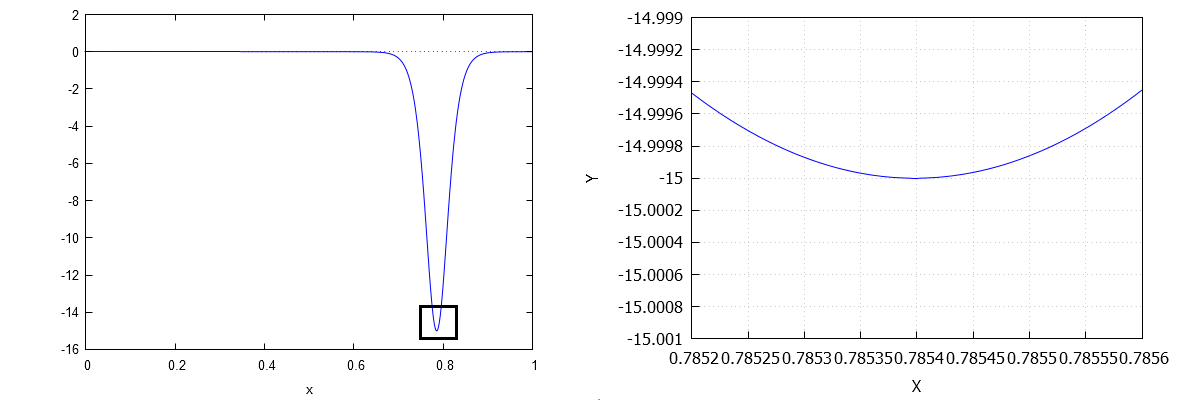
\includegraphics[scale = 0.47]{figure1.png}
    \caption*{Gráfico da derivada da função $f(x)$.}
  \end{center}
\end{figure}
\begin{flushleft}
  \textbf{Resolução Teórica:}
\end{flushleft}
\hspace{10mm}Se a função $f'(x) = (\frac{\cos(x)^{30}}{\sin(x)^{30}+\cos(x)^{30}})' $ for contínua em [a,b], então o erro absoluto majorado cometido ao usar a regra dos retângulos composta é dado por: $$\exists t\in]a,b[\text{ : } \left|E_{n}^{R}\right| = \left|\frac{b-a}{2}h\times f'(t)\right| \leq \frac{b-a}{2}h\times M $$ onde $M = max_{a\leq x \leq b}|f'(x)|$.
Com apoio ao gráfico antecedente, obtivemos o valor $M \leq 15.001$\footnote{Mesmo com o valor obtido "longe" do máximo, apenas afetará o número de iterações na ordem dos milhares o que, do ponto de vista computacional, é praticamente irrelevante e, portanto, decidimos utilizá-lo mesmo assim.}.\\[5mm]
\textbf{Resposta:}
\begin{itemize}
  \item{\textbf{$7$ casas decimais corretas:}\\[2mm]
  \textbf{Cálculo de n:} \par Tem-se que $[a,b] = [0,1]$ e M = 15.001. Como se pretende calcular o valor de I com 7 casas decimais corretas, $\epsilon = 5\times 10^{-8}$. Com isto, $\left|\frac{1}{2}h\times M \right| = \left|\frac{1}{2}\times \frac{1}{n} \times M \right|\leq 5\times10^{-8}$ e, portanto, $n > M\times \frac{(1)^{2}}{10\times 10^{-8}}$. Basta $ n = 150010001$. \\[2mm]
  \textbf{Output do programa:}
  \begin{lstlisting}[language=Python]
  >>> I_r(5*10**-8)
  Extremo esquerdo (a): 0
  Extremo direito (b): 1
  Maximo da derivada em [a,b]: 15.001
  n = 150010001
  Integral = 0.785398140941796 Tempo execucao: 360.9465343952179  \end{lstlisting}
  \textbf{Valor de I:} $0.785398141 \pm 5\times10^{-8}$.}\\[2mm]
  \textbf{Nota:} Visto que o $\epsilon$ máquina está na ordem de grandeza de $10^{-16}$, ao executar n iterações, o erro da máquina aumentará para $n\times\epsilon\approx1.7\times10^{-8}$, o que torna calcular aproximações com mais do que 7 casas decimais corretas não exequível.
  \newpage
  \item {\textbf{$12$ casas decimais corretas:}\\[2mm]
  \textbf{Cálculo do n:}
  É análogo a 7 casas decimais, mas, agora, $n > M\times \frac{(1)^{2}}{10\times 10^{-13}}$, ou seja, basta $ n = 15001000000001$. Uma vez que para $5\times10^{8}$ demorou 360 segundos a correr, é de esperar que para $1.5\times10^{13}$ demore cerca de 36000000 segundos, ou seja, 416 dias. Para além disso, tal como mencionado na nota anterior, o erro máquina, com este número de iterações, será superior a $10^{-8}$ o que dificulta o cálculo pedido. Como tal, decidimos calcular o valor do integral com 6 casas decimais corretas.\\[2mm]
  \textbf{Output do programa:}
  \begin{lstlisting}[language = Python]
  >>> I_r(5*10**-7)
Extremo esquerdo (a): 0
Extremo direito (b): 1
Maximo da derivada em [a,b]: 15.001
n = 15001001
Integral = 0.7853981715131676 Tempo de execucao: 28.726349353790283\end{lstlisting}
\textbf{Valor de I:} $0.78539817\pm5\times10^{-7}$
}\end{itemize}
\textbf{Comentários:}\\
Após a resolução da parte 1 do trabalho, observámos alguns aspetos notáveis. Tais como:
\begin{itemize}
  \item{A nível computacional, é um método com uma implementação básica o que permite tornar este método rápido de implementar numa dada linguagem.}
  \item{Uma vez que o majorante do erro é inversamente proporcional à amplitude de cada subintervalo, torna-se muito demorado pois, se para um dado erro $\epsilon$ demora $n$ iterações, para $\epsilon\times10^{-1}$ demoraria $10\times n$ iterações. Ou seja, é um crescimento exponencial o que não é otimal.}
\end{itemize}

\section*{Exercício 2.}
\textbf{Código utilizado:}
\begin{lstlisting}[language=Python]
def f(x):
    return cos(x)**30/(sin(x)**30+cos(x)**30)

def I_s(a,b):
    par = 0
    impar = 0
    for k in range(20):
        I = 0
        par += impar
        impar = 0
        n = 2**k
        h = abs(b-a)/(2*n)
        for j in range(n):
            impar += f((a+h)+2*h*j)
        I += f(a)+ f(b) + 4*impar + 2*par
        print('k =', k, 'Integral =', h*I/3, '|I-In| =', abs(Valor_Integral-h*I/3))

Valor_Integral = 0.785398138155361
\end{lstlisting}
\textbf{Observações:} O código que utilizámos foi feito de modo a que, para calcular um integral entre $[a,b]$ considerando $n$ intervalos, $n\in2\mathbb{N}$, é necessário introduzir $\frac{n}{2}$ no input do programa. Isto deve-se ao facto de, dado um \textit{input} $n$ de intervalos, o programa irá dividir o intervalo $[a,b]$ em $n$ subintervalos e, depois, calcular os pontos médios de cada um desses intervalos. Ou seja, irá dividir cada um dos subintervalos em dois subsubintervalos de igual amplitude.\\[5mm]
\textbf{Tabela:}
\begin{center}
\begin{tabular}{c|c|c}
  k & $I_{n_{k}}$ & $|I-I_{n_{k}}|$ \\
  \hline
  1 & 0.8333336061785755 & 0.04793546802321458 \\
  2 & 0.8811244340152541 & 0.09572629585989312 \\
  3 & 0.7835174103225927 & 0.0018807278327682697 \\
  4 & 0.7800452773015049 & 0.005352860853856112 \\
  5 & 0.7855479919341913 & 0.00014985377883036666 \\
  6 & 0.78539677204528 & 1.3661100809470028e-06 \\
  7 & 0.7853981380977532 & 5.7607807413262435e-11 \\
  8 & 0.7853981381547627 & 5.982991879704969e-13 \\
  9 & 0.7853981381553234 & 3.752553823233029e-14 \\
  10 & 0.785398138155359 & 1.9984014443252818e-15 \\
  11 & 0.7853981381553604 & 5.551115123125783e-16 \\
  12 & 0.7853981381553606 & 3.3306690738754696e-16 \\
  13 & 0.7853981381553621 & 1.1102230246251565e-15 \\
  14 & 0.7853981381553593 & 1.6653345369377348e-15 \\
  15 & 0.7853981381553631 & 2.1094237467877974e-15 \\
  16 & 0.7853981381553617 & 7.771561172376096e-16 \\
  17 & 0.7853981381553705 & 9.547918011776346e-15 \\
  18 & 0.7853981381553877 & 2.6756374893466273e-14 \\
  19 & 0.7853981381553989 & 3.7969627442180354e-14 \\
  20 & 0.7853981381554388 & 7.782663402622347e-14 \\
  \hline
\end{tabular}
\end{center}
\par
\textbf{Comentários:}\par
Após uma análise dos valores obtidos, verificámos que, apartir de $n=2^k, k>9$, já não conseguimos determinar a precisão com que a regra de simpson calcula o valor do integral. Isto deve-se ao facto de apenas temos obtido um valor do integral com erro na ordem de grandeza $10^{-14}$. Para valores de $k>9$, observam-se oscilações entre os erros absolutos. Para isto determinamos duas possíveis causas:
\begin{enumerate}
  \item{Tal como exposto anteriormente, o valor de $I$ que utilizámos tem um erro associado de $10^{-14}$ o que impossibilita o cálculo de $|I-I_{n_k}|$ para $k>9$ e pode causar a tal oscilação de valores do mesmo.}
  \item{Visto que o $\epsilon$ máquina está na ordem de grandeza de $10^{-16}$, é impossível calcular $I_{n_k}$ com erro inferior a $10^{-16}$. Como, para $k=9$, o erro está na ordem de grandeza de $10^{-14}$, podemos conjeturar que o erro decresce rapidamente e é provável que com cálculos mais precisos, o erro associado a $k>9$ esteja na ordem de grandeza de $10^{-16}$ o que, tal como explicado, já não nos é possível com o sistema de vírgula flutuante em uso.}
\end{enumerate}
\section*{Conclusões}
\hspace{10mm}Ao realizar este trabalho, conseguimos tirar algumas conclusões relativamente aos dois tipos de integrações numéricas utilizados: regra retângulos e regra de simpson compostas.
\begin{itemize}
  \item{\textbf{Regra retângulos: }Um método de fácil compreensão e implementação que requer poucos gastos computacionais, mas com uma otimização bastante baixa, uma vez que é necessário realizar um grande número de iterações para encontrar aproximações de integrais com erros relativamente baixos. É bastante fácil de determinar um majorante do erro e apenas requer que a função a integrar seja de classe $C^1$ para tal.}
  \item{\textbf{Regra Simpson: }Um método com uma compreensão e implementação mais complexa, comparando com a regra dos retângulos, mas com uma precisão bastante superior, uma vez que foram apenas necessárias cerca de 1024 iterações (cada iteração por subintervalo) para encontrar uma aproximação do integral com um erro bastante baixo. Contrariamente à regra dos retângulos, para o cálculo de majoração do erro já exige mais da função a integrar, classe $C^4$, e torna-se mais complicado de majorar o mesmo.}
\end{itemize}
Em suma, ambas as regras têm as suas vantagens e desvantagens, mas, mais geralmente, será mais benéfico a utilização da regra de simpson uma vez que não requer um custo temporal tão elevado.
\end{document}
